\documentclass[tikz, border=3mm]{standalone}
\usepackage{tikz}
\usetikzlibrary{arrows.meta, calc} % For arrow tips and coordinate calculations

\begin{document}
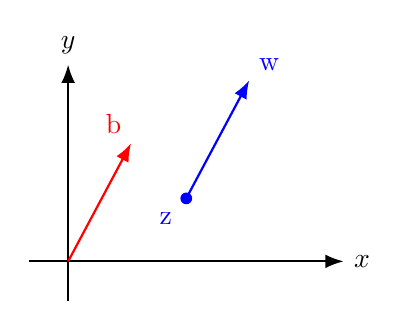
\begin{tikzpicture}[
    >=Latex, % Set default arrow tip style
    vector/.style={->, thick}, % Style for vectors
    dot/.style={fill=blue, circle, inner sep=1.5pt} % Style for the point z
]

    % Axes
    \draw[->, thick] (-0.5, 0) -- (3.5, 0) node[right] {$x$}; % Added x label for context
    \draw[->, thick] (0, -0.5) -- (0, 2.5) node[above] {$y$}; % Added y label for context

    % Define vector b displacement and endpoint
    \coordinate (b_vec) at (0.8, 1.5); % Displacement vector for b (and w)
    \coordinate (b_end) at (b_vec);    % Endpoint of b (starts at origin)

    % Draw Red Vector 'b'
    \draw[vector, red] (0,0) -- (b_end);
    \node[red, above left] at (b_end) {b}; % Label near endpoint

    % Define start point z
    \coordinate (z) at (1.5, 0.8);

    % Calculate endpoint w using z and the displacement vector b_vec
    \coordinate (w) at ($(z) + (b_vec)$);

    % Draw Blue Vector 'w' from 'z'
    % Add the point indicator at z first
    \node[dot, label={[blue]below left:z}] at (z) {}; % Apply dot style and label
    % Draw the vector starting from z
    \draw[vector, blue] (z) -- (w);
    \node[blue, above right] at (w) {w}; % Label end point w

\end{tikzpicture}
\end{document}